% Assignment 1
\documentclass{article}
\usepackage[left=2cm, right=2cm, top=2cm]{geometry}
%%%%%%%%%%%%%%%%%%%%%%%%%%%%%%%%%% PACKAGES %%%%%%%%%%%%%%%%%%%%%%%%%%%%%%%%%%
\usepackage{graphicx}                   % PNGs
\usepackage{hyperref}                   % Hyperlinks
\usepackage{amsmath}
\usepackage{algorithm}                  % Algorithms
\usepackage{algpseudocode}              % Algorithms
\usepackage{pdfpages}                   % Include PDFs

\hypersetup{
    colorlinks,
    linkcolor=black
}

%%%%%%%%%%%%%%%%%%%%%%%%%%%%%%%%%%%%%%%%%%%%%%%%%%%%%%%%%%%%%%%%%%%%%%%%%%%%%%%

\pagenumbering{gobble}

\title{\textbf{Assignment \#1}}
\author{MacMillan, Kyle}
\date{October 10, 2018}


\begin{document}

\maketitle
\addcontentsline{toc}{section}{Title}

\newpage
\pagenumbering{roman}   % Set TOC page numbering to lowercase roman numerals
\tableofcontents
\addcontentsline{toc}{section}{Table of Contents}

\newpage
\listoffigures
\addcontentsline{toc}{section}{List of Figures}

% \listofalgorithms
% \addcontentsline{toc}{section}{List of Algorithms}

\newpage
\pagenumbering{arabic}  % Set content page numbering to arabic numerals
% Setup Hyperlinks for the rest of the document
\hypersetup{
    citecolor=blue,
    filecolor=black,
    linkcolor=blue,
    urlcolor=blue
}

\setcounter{page}{1}
\section[Problem 1]{Briefly explain the difference between}
\subsection[Compilers and Interpreters]{A compiler and an interpreter}
Compilers are different from interpreters or they would not be separate things. 
In general terms a compiler takes something and turns it into something else. 
An interpreter does the same thing but not as efficiently. The compiler we use 
to compile C\texttt{++} will read through our code and reduce it to assembly 
instructions for the machine we are on. While doing this it will evaluate some 
parts of the code and place things in an ``optimal'' ordering. An interpreter 
does not look at the code until execution, meaning it has no room to perform 
optimizations. Another difference is that interpreters are able to take code on 
the fly, whereas a compiled language must have everything at compile time. 

\subsection[Statically and Dynamically Typed Languages]{A statically typed 
language and a dynamically typed language}
Statically typed languages strictly enforce \textit{type}, whereas dynamically 
typed languages determine which \textit{type} to use. There are two primary 
benefits to statically typed languages:\\
\begin{itemize}
    \item type-safe -- You must declare the type and it will be enforced
    \item speed -- Knowing the type ahead of time means it doesn't have to 
    figure it out on the fly
\end{itemize}

A dynamically typed language is able to determine the type on the fly which 
reduces development time but can also be confusing. In Python, for example, a 
function with a variable named ``flow''. A user may not initially know if flow 
is a string such as \textit{`fast', `normal'} or \textit{`slow'}, or a float 
such as a flow rate. This confusion can make maintenance more difficult. It can 
also hamper someone trying to learn the codebase. There are pros and cons of 
both that need to be taken into consideration when choosing a language.

\subsection[JIT Compiler and Interpreters]{A just-in-time compiler and an 
interpreter}
A just-in-time (JIT) compiler compiles as you send it commands, meaning at 
runtime. A JIT, such as what Java uses, will take the code and compile it to 
bytecode. An interpreter executes instructions. A JIT will have marginally 
better performance compared to an interpreter.

\subsection[Top-Down and Bottom-Up Parsing]{Top-down parsing and bottom-up 
parsing}
Top-down (TD) and bottom-up (BU) parsing refers to the methods of constructing 
a parse tree. As can be assumed, they each begin at their respective ``ends'' 
of a tree. TD parsers can be attacked with a predictive \textit{LL(k)} method 
where \textit{LL} means it descends the left nodes and has a look-ahead of 
\textit{k}. BU parsing involves constructing a parse tree from a given input by 
starting at the bottom, ascending towards the root. BU parsing can use a 
shift-reduce method where the input string is reduced by shifting out the 
left-most element of the input to be evaluated. A tool for both Top-Down and 
Bottom-Up parsers is the \textbf{FIRST} and \textbf{FOLLOW} method.




\newpage
\section[Problem 2]{Let L be the language \{$abxba$ $\vert$ $x$ is any string 
of $a$'s, $b$'s, and $c$'s not containing the substring $ba$\}}
\subsection[Minimum-State DFA]{Construct a minimum-state deterministic finite 
automaton for L}
Any string of $a$'s, $b$'s, and $c$'s not containing the substring $ba$ could 
be rewritten as $x = (a^\ast b^\ast c^\ast)^\ast$ where $x$ contains every set 
combination of $a$'s, $b$'s, and $c$'s such that $\{ba\} \cap x = \varepsilon$. 
In order for $ba$ to not intersect $x$ we have to ensure the minimum-state DFA 
cannot go from $b \to\ a$. The visualization is dentoted in Figure \ref{p1:dfa}. 
Blue denotes the $x$ section and orange are empty sets. Of special note is that 
where $b$ terminates it cannot pass \varepsilon.

\begin{figure}[hc]
\centering
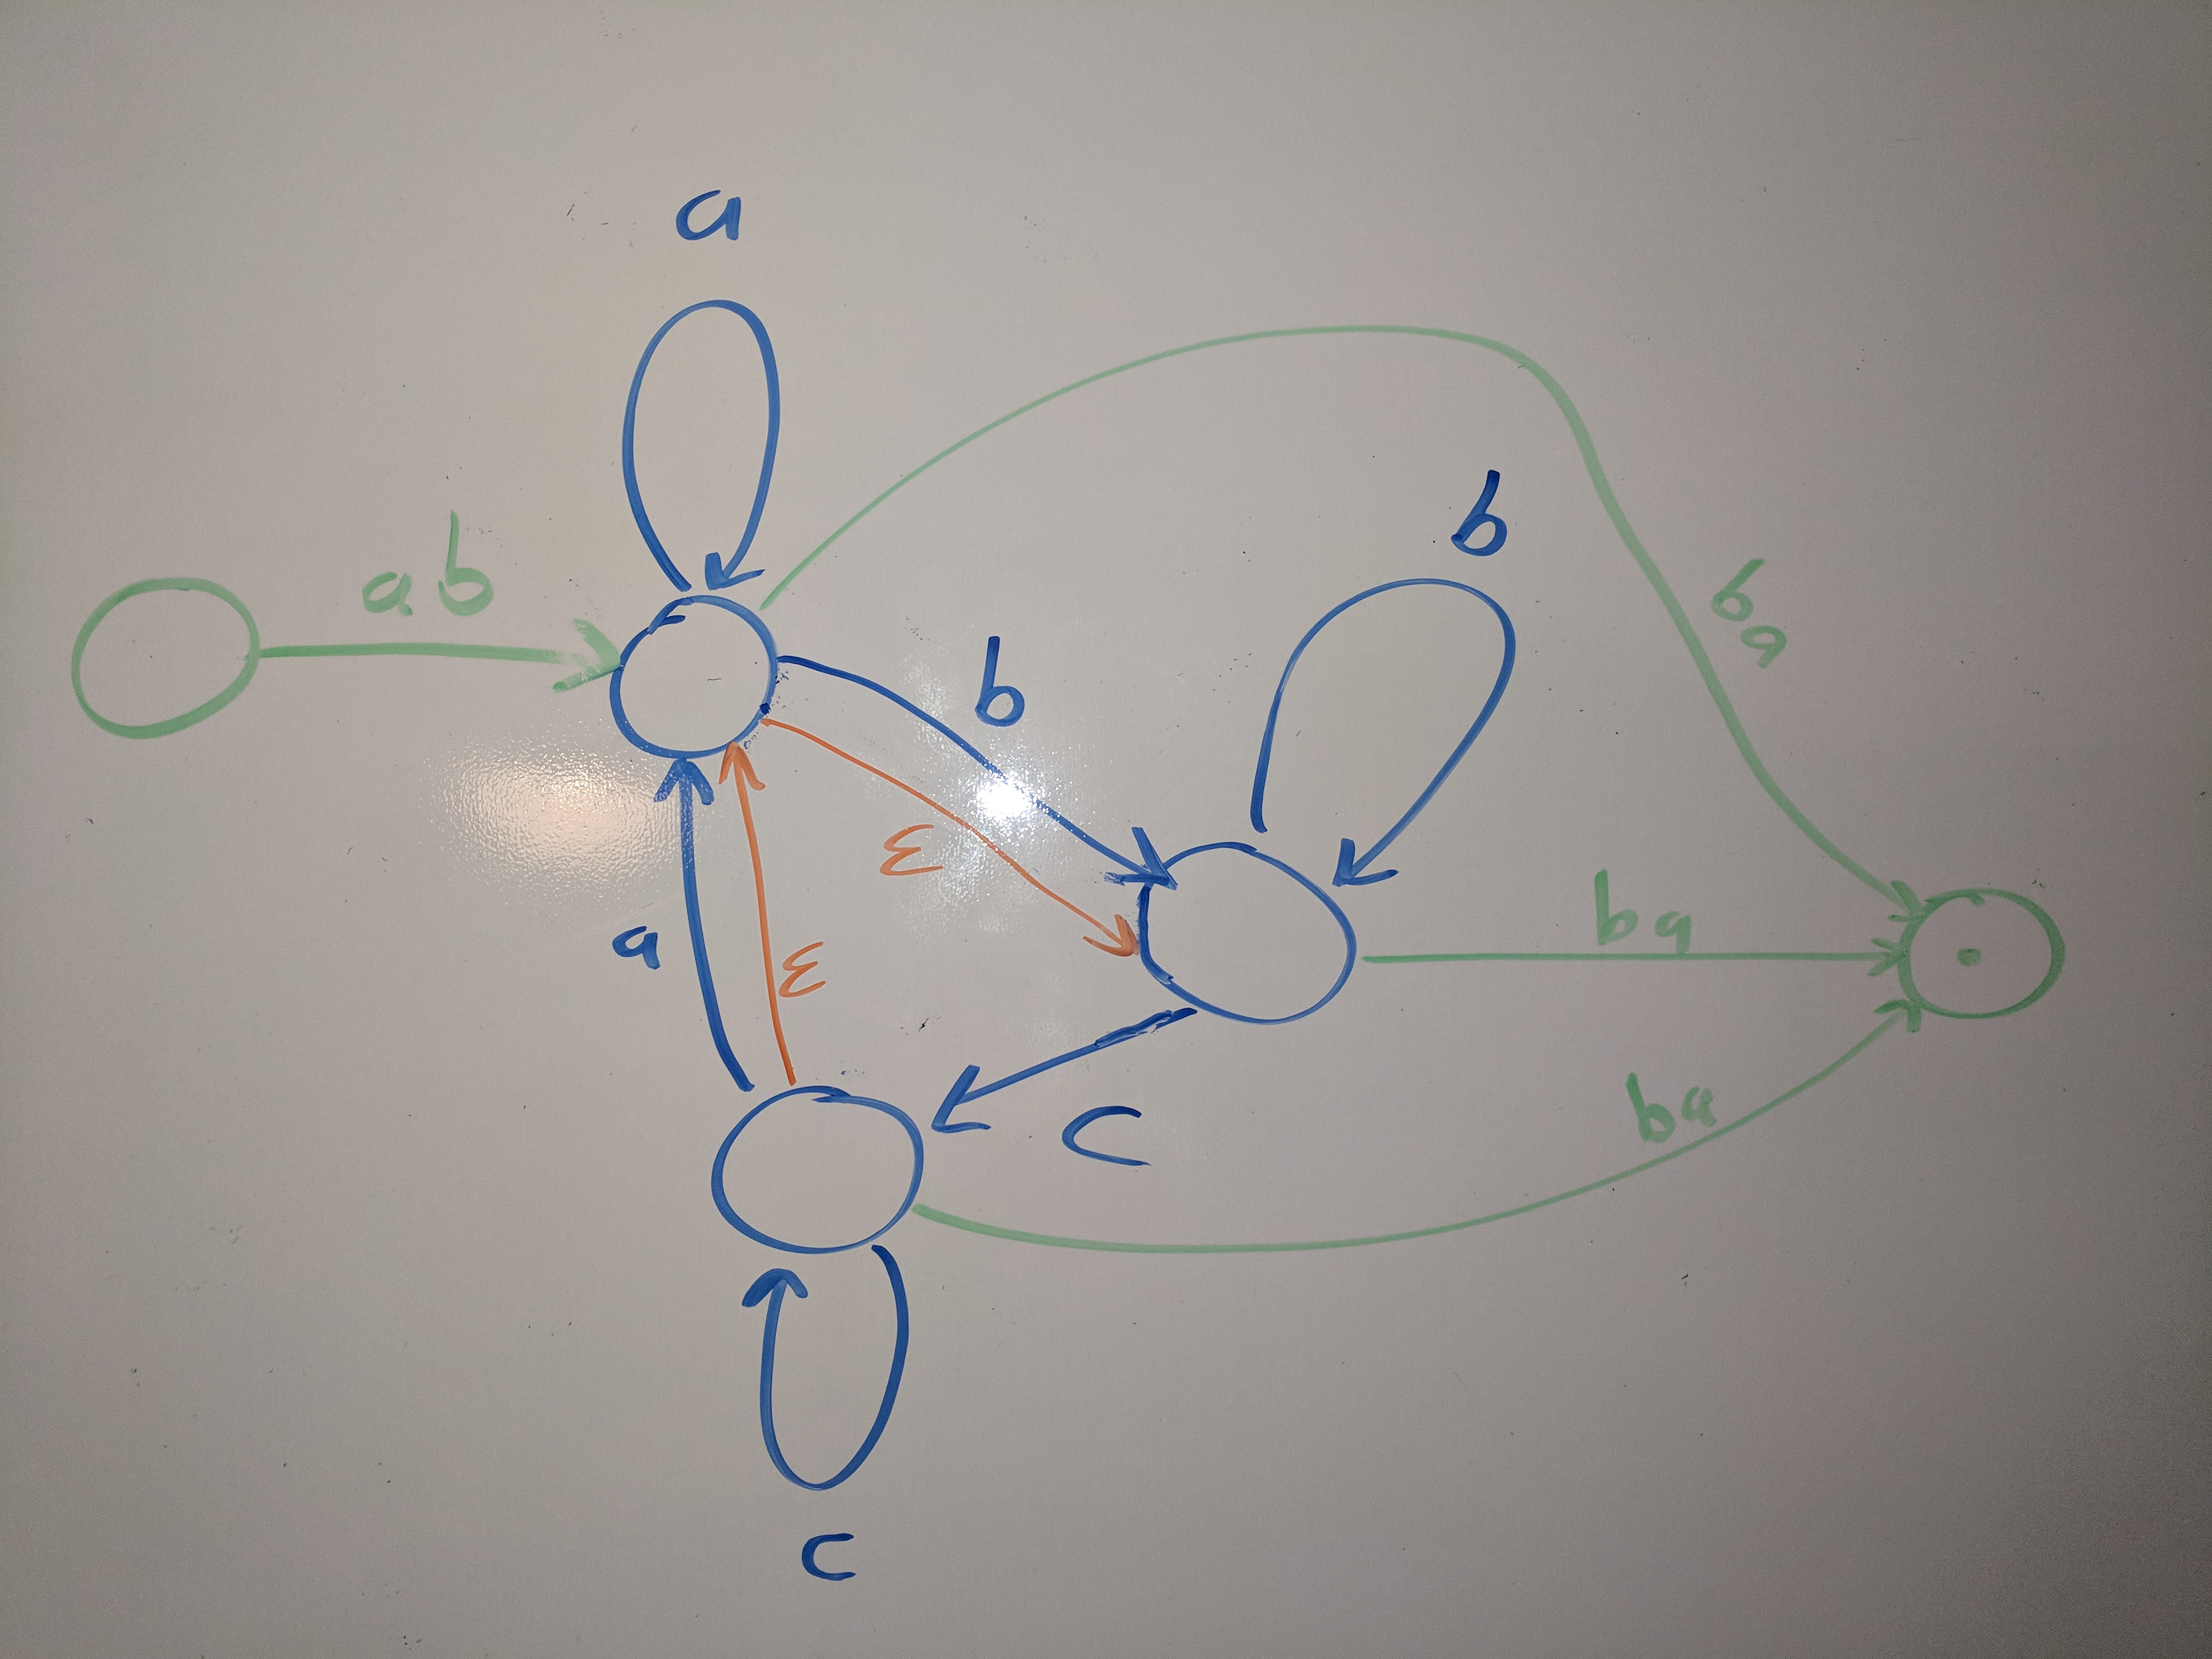
\includegraphics[width=0.5\textwidth]{images/p2-1}}
\caption{Minimum-State DFA}
\label{p1:dfa}
\end{figure}


\subsection[Input String: abbcabcba]{Show how your DFA processes the input 
string abbcabcba}
filler

\subsection[Input String: abbcababa]{Show how your DFA processes the input 
string abbcababa}
filler

\subsection[Regular Expression for L]{Construct a regular expression for L}
filler

\subsection[Regular Expression generate: abbcabcba]{Show how your regular 
expression generates the input string abbcabcba}
filler





\newpage
\section[Problem 3]{Let L be the set of all strings of a's and b's with the 
same number of a's as b's}
\subsection[LL1 Grammar]{Construct an LL(1) grammar that generates L}

\subsection[Generation Explanation]{Explain how your grammar generates L}

\subsection[Proof of LL(1)]{Prove that your grammar is LL(1) }

\subsection[Predictive Parser]{Construct a predictive parsing table for your 
grammar }

\subsection[Predictive Parser: abbbaa]{Show how your predictive parser 
processes the input string abbbaa }




\newpage
\section[Problem 4]{Interactive desk calculator for prefix expressions}
\subsection[Lex/Yac Interpreter]{Using Lex and Yacc or their equivalents, 
implement an interpreter that evaluates newline-terminated input lines of 
prefix arithmetic expressions. The expressions may contain integers and 
operators for addition, subtraction, multiplication, division, and negation. 
The answers are to be integers. Show the Lex-Yacc code for your calculator}
\subsection[Calculator Output]{Show the output generated by your calculator for}

\begin{tabular}{ll}
\indent 1. \texttt{+ 1 - 2 3} & output1 \\
\indent 2. \texttt{+ 1 - 2} & output2 \\
\end{tabular}






\newpage
\section[Problem 5]{A Turing machine is an abstract computer that can do any 
computation that a real computer can do. Because the Turing machine is an 
abstract machine, it does not have the physical properties that a real machine 
has. For example, its tapes are infinite (or at least unbounded for purposes of 
any particular calculation) in length. Another important characteristics is 
that it lacks a clock that is tied to time in the real world.}
\subsection[Turing Machine Double Click]{Explain how a Turing machine can 
detect the fact that two mouse clicks occur close together in real-world time 
even though it has no clock.}
While the proposed machine does not have a clock, it will do computations, and 
computations are discretizations. A turing machine can have an interger symbol 
that counts the number of times it's able to add one to the symbol between key 
presses, resetting the symbol after checking for a double click. If the symbol 
value is in a predefined range it would be considered to be in the state of a 
double-click. In order to qualify as a Turing Machine actions must be finite, 
\textbf{discrete}, and distinguishable; memory is infinite, and it can run 
until after the universe dies. So you can have arbitrarily ``long'' periods of 
time between clicks.


\end{document}
